% SC4063 --- Chapter 1: Threat Landscape and Attack Surface (0->100)
\chapter{Threat Landscape and Attack Surface}\label{ch:threatnet}
\sloppy

\begin{quote}
\emph{``You cannot defend what you cannot see.''} --- The first job of network
security is to draw an honest map: who wants in, where the doors are, and what
lies behind each one.
\end{quote}

\noindent\fbox{\parbox{\dimexpr\linewidth-2\fboxsep-2\fboxrule}{%
\textbf{From zero: no security background assumed.} We start from a house with
doors and valuables, turn it into packets on a wire, and build the vocabulary
of assets, adversaries, and attack surfaces from scratch. Every term is defined
on first use, picture first, then formalism. This chapter is the lens for the
whole book.}}
\vspace{0.4em}

\section*{Learning Outcomes}
After this chapter you will be able to:
\begin{enumerate}[label=(L\arabic*)]
    \item model the network adversary (Dolev--Yao, insider, APT) and its capabilities;
    \item define \emph{attack surface} and enumerate it from a network diagram;
    \item map STRIDE/CIA threats to OSI/TCP-IP layers;
    \item apply defence-in-depth, least privilege, and zero-trust reasoning;
    \item prioritise controls with qualitative risk and CVSS intuition.
\end{enumerate}

% ============================================================
\section{Who Is the Adversary?}\label{sec:adversary}
Intuition first. A house assumes burglars exist; a network must assume the
\emph{road itself} is hostile. Packets travel over fibre, Wi-Fi, and routers
you do not control. The strongest useful abstraction is the
\emph{Dolev--Yao} attacker: she can \emph{eavesdrop} every packet, \emph{modify}
or \emph{inject} any packet, \emph{replay} old packets, and \emph{drop}
packets at will, but cannot break cryptography without the key.

\begin{definition}[Network adversary]\label{def:adversary}
The \emph{Dolev--Yao} adversary controls the network: read, modify, inject,
replay, and drop. An \emph{insider} is an authorised user who abuses privilege.
An \emph{advanced persistent threat} (APT) is a well-resourced actor who
combines network, host, and social vectors over months. All three are
assumed to be active simultaneously.
\end{definition}

Why assume such power? Because the Internet delivers it cheaply: a café Wi-Fi
lets anyone sniff, a compromised router lets anyone modify, and botnets let
anyone flood. Designing for a weaker attacker yields a system that fails the
day someone stronger appears. Cryptography is the only edge case where the
adversary is bounded: without the key, a ciphertext looks random.

Threat actors differ in motive, resources, and stealth. A script kiddie runs
ready-made exploits for fun; a criminal syndicate monetises data; a
nation-state seeks persistence and deniability. The network sees the same
SYN scan from all three, but the follow-up differs: the first stops, the
second deploys ransomware, the third implants a backdoor that beacons slowly.

\begin{example}[Coffee-shop attack]\label{ex:cafe}
Alice joins \texttt{Free\_WiFi}, opens \texttt{http://intranet.corp/}. The
attacker runs \texttt{arpspoof} to become the gateway, strips the redirect to
HTTPS, and sees Alice's cookie. Dolev--Yao predicted every step: eavesdrop,
inject (ARP), modify (strip), replay (cookie). TLS (Ch.~4/8) would have made
the ciphertext useless, but only if Alice had verified the certificate.
\end{example}

% ============================================================
\section{Attack Surface: Where Can They Enter?}\label{sec:surface}
An \emph{asset} is what you protect (data, service, reputation); an
\emph{attack surface} is the set of points where untrusted data can enter or
trusted data can leave. Smaller surface means fewer places to be wrong.

\begin{definition}[Attack surface]\label{def:surface}
The \emph{attack surface} of a networked system is the set
$\mathcal{S}= (E,F,T)$ of \emph{entry points} $E$ (open ports, APIs, wireless
SSIDs), \emph{flows} $F$ (packet paths between trust zones), and \emph{trust
boundaries} $T$ where privilege changes. Each element of $\mathcal{S}$ is an
opportunity to apply STRIDE analysis.
\end{definition}

Draw it. Start with a data-flow diagram: external entities (Internet,
partner), processes (web server, DB), stores (DB, object storage), and flows
(arrows). Dashed lines mark trust boundaries; every crossing is a candidate
entry. Then count: each open TCP port, each UDP service, each SSID, each
VPN endpoint adds one entry. The perimeter is not one line but many: edge
router, WAF, Wi-Fi, and every laptop that leaves the building.

\begin{figure}[h]\centering
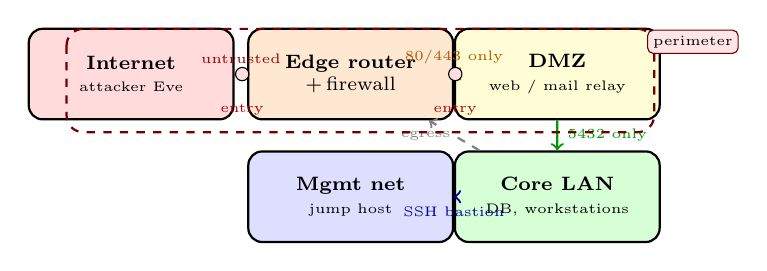
\begin{tikzpicture}[scale=0.82, every node/.style={font=\scriptsize},
  zone/.style={draw,thick,rounded corners=5pt,minimum width=2.6cm,minimum height=1.15cm,align=center}]
\node[zone,fill=red!14] (inet) at (0,2.85) {\textbf{Internet}\\\tiny attacker Eve};
\node[zone,fill=orange!18] (edge) at (3.4,2.85) {\textbf{Edge router}\\+\,firewall};
\node[zone,fill=yellow!16] (dmz) at (6.6,2.85) {\textbf{DMZ}\\\tiny web / mail relay};
\node[zone,fill=green!16] (core) at (6.6,0.95) {\textbf{Core LAN}\\\tiny DB, workstations};
\node[zone,fill=blue!13] (mgmt) at (3.4,0.95) {\textbf{Mgmt net}\\\tiny jump host};
\draw[->,thick,red!60!black] (inet) -- (edge) node[midway,above,font=\tiny] {untrusted};
\draw[->,thick,orange!70!black] (edge) -- (dmz) node[midway,above,font=\tiny] {80/443 only};
\draw[->,thick,green!60!black] (dmz) -- (core) node[midway,right,font=\tiny] {5432 only};
\draw[->,thick,blue!60!black] (mgmt) -- (core) node[midway,below,font=\tiny] {SSH bastion};
\draw[->,thick,dashed,gray] (core) -- (edge) node[midway,left,font=\tiny,fill=white,inner sep=1pt] {egress};
\draw[thick,red!45!black,dashed,rounded corners=6pt] (-1.0,3.55) rectangle (8.1,1.95);
\node[font=\tiny,fill=red!10,rounded corners=2pt,inner sep=2pt,draw=red!40!black] at (8.7,3.35) {perimeter};
\node[draw,fill=red!12,circle,inner sep=1.7pt] at (1.72,2.85) {}; \node[font=\tiny,red!70!black] at (1.72,2.30) {entry};
\node[draw,fill=red!12,circle,inner sep=1.7pt] at (5.02,2.85) {}; \node[font=\tiny,red!70!black] at (5.02,2.30) {entry};
\end{tikzpicture}
\caption{Network perimeter with trust boundaries. Red dots are entry points where attacker-controlled packets cross inward. Every crossing needs a threat class and a control.}
\label{fig:perimeter}
\end{figure}

\begin{figure}[h]\centering
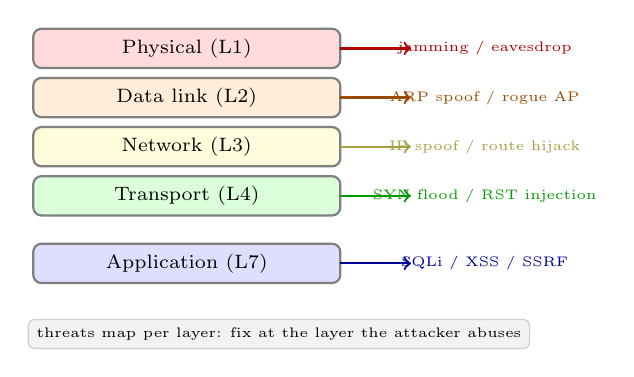
\begin{tikzpicture}[scale=0.78, every node/.style={font=\scriptsize}]
\foreach \y/\lab/\col in {5.2/Physical (L1)/red!14,4.4/Data link (L2)/orange!14,3.6/Network (L3)/yellow!14,2.8/Transport (L4)/green!14,1.7/Application (L7)/blue!13} {
  \draw[fill=\col,draw=black!50,thick,rounded corners=3pt] (0,\y-0.32) rectangle (5.0,\y+0.32) node[midway] {\lab};
}
\foreach \y/\txt/\col in {5.2/{jamming / eavesdrop}/red!70!black,4.4/{ARP spoof / rogue AP}/orange!60!black,3.6/{IP spoof / route hijack}/yellow!60!black,2.8/{SYN flood / RST injection}/green!60!black,1.7/{SQLi / XSS / SSRF}/blue!60!black} {
  \node[font=\tiny,align=left,text=\col] at (7.35,\y) {\txt};
  \draw[->,thick,\col] (5.0,\y) -- (6.15,\y);
}
\node[font=\tiny,fill=gray!10,rounded corners=2pt,inner sep=3pt,draw=gray!40] at (4.0,0.55) {threats map per layer: fix at the layer the attacker abuses};
\end{tikzpicture}
\caption{OSI/TCP-IP layer vs.\ threat badge. Lower layers attack availability and authenticity; upper layers attack confidentiality and integrity.}
\label{fig:layer-threat}
\end{figure}

Reducing surface is engineering: close unused ports, put the DB on a private
subnet with no Internet route, enforce egress filtering (compromised hosts
should not call home on arbitrary ports), and treat every laptop's Wi-Fi as
untrusted even inside the office. A VPN (Ch.~4) does not shrink the surface;
it moves it to the VPN gateway, which must then be hardened.

\begin{lstlisting}[language=Python,caption={Enumerating the network attack surface from a simple port scan.},label={lst:surface}]
import socket
TARGETS = ["10.0.0.5","10.0.0.12","10.0.2.8"]
PORTS   = [22,80,443,5432,6379]  # candidates to probe
surface = []
for host in TARGETS:
    for port in PORTS:
        s = socket.socket(); s.settimeout(0.4)
        if s.connect_ex((host, port)) == 0:  # open
            surface.append((host, port))
        s.close()
print(f"attack surface: {surface}")
# -> [('10.0.0.5', 22), ('10.0.0.5', 443), ('10.0.2.8', 5432)]
# Each tuple is an entry point that needs a STRIDE row.
\end{lstlisting}

% ============================================================
\section{Threat Classification and Risk}\label{sec:stride}
STRIDE partitions threats by the property violated: Spoofing (authenticity),
Tampering (integrity), Repudiation, Information disclosure (confidentiality),
Denial of service (availability), Elevation of privilege (authorisation).
Apply it per flow: a packet crossing the Internet$\to$DMZ invites S/T/I/D; a
DB query from DMZ$\to$core invites T/I/E.

Risk prioritises the list. Qualitatively,
$\text{Risk}=\text{Likelihood}\times\text{Impact}$ on a $3\times3$ matrix;
quantitatively, CVSS v3 scores 0--10 from exploitability and impact metrics.
A reflected XSS on an internal tool may be medium; unauthenticated RCE on the
DMZ web server is critical (CVSS 9.8) and fixed before release.

\begin{figure}[h]\centering
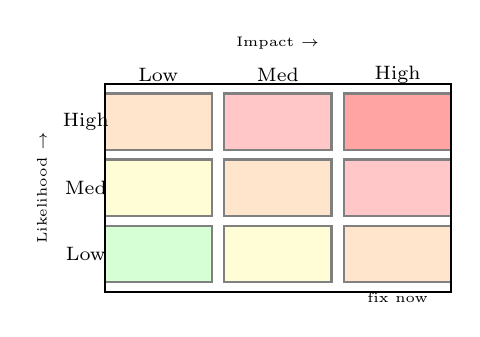
\begin{tikzpicture}[scale=0.80, every node/.style={font=\scriptsize}]
\foreach \x/\y/\col/\txt in {1.0/1.0/green!16/low$\times$low,2.9/1.0/yellow!16/low$\times$med,4.8/1.0/orange!20/low$\times$high,1.0/2.05/yellow!16/med$\times$low,2.9/2.05/orange!20/med$\times$med,4.8/2.05/red!22/med$\times$high,1.0/3.1/orange!20/high$\times$low,2.9/3.1/red!22/high$\times$med,4.8/3.1/red!36/high$\times$high} {
  \fill[\col,draw=black!50,thick] (\x-0.85,\y-0.45) rectangle (\x+0.85,\y+0.45) node[midway,align=center,font=\tiny] {\txt};
}
\foreach \x/\lab in {1.0/Low,2.9/Med,4.8/High} \node at (\x,3.85) {\lab};
\foreach \y/\lab in {1.0/Low,2.05/Med,3.1/High} \node at (-0.15,\y) {\lab};
\node[font=\tiny,above] at (2.9,4.10) {Impact $\to$}; \node[font=\tiny,rotate=90] at (-0.85,2.05) {Likelihood $\to$};
\node[font=\tiny,fill=white,rounded corners=2pt,inner sep=2pt] at (4.8,0.30) {fix now};
\draw[thick] (0.15,0.40) rectangle (5.65,3.70);
\end{tikzpicture}
\caption{Risk heatmap (likelihood $\times$ impact). Colour deepens toward critical. CVSS refines each axis into exploitability and impact sub-scores.}
\label{fig:risk}
\end{figure}

Two principles guide controls. \emph{Defence in depth} means an attacker must
defeat several independent controls (firewall + IDS + TLS + auth). \emph{Least
privilege} means each flow is allowed the narrowest 5-tuple that still serves
its purpose. Zero trust pushes both to the limit: never trust the network,
always authenticate and authorise per flow. The perimeter becomes a set of
micro-perimeters around every service.

\begin{remark}[Threat modelling is iterative]\label{rem:iter}
Every feature adds flows and stores. ``Add OAuth'' adds a redirect flow that
crosses the trust boundary twice; ``allow file upload'' adds storage and a
rendering flow in another user's browser. Re-run STRIDE on the delta; if the
cheapest attack path after the fix is not strictly more expensive, the fix was
cosmetic. Models that do not evolve become fiction.
\end{remark}

% ============================================================
\section{Exercises}\label{sec:ch01-exercises}
\begin{enumerate}[label=E1.\arabic*, leftmargin=*, itemsep=0.6em]
    \item \textbf{Dolev--Yao trace.} Alice sends $m$ over Wi-Fi to Bob. List five
    distinct actions a Dolev--Yao attacker can take on that single transmission
    and name the CIA property each violates.
    \item \textbf{Attack surface enumeration.} Draw a DFD for a campus app:
    mobile$\to$API gateway$\to$app service$\to$DB, plus push notifications to
    recipients. Mark trust boundaries, list every entry point, and identify the
    entry with highest asset exposure. Propose one reduction.
    \item \textbf{STRIDE per layer.} For the flow \texttt{client}$\to$\texttt{CDN}$\to$\texttt{origin}$\to$\texttt{DB},
    enumerate which STRIDE letters apply at each hop. Give one concrete exploit
    per letter that actually applies; omit letters that do not.
    \item \textbf{Risk scoring.} Score two threats with CVSS intuition: (a) reflected
    XSS on search and (b) unauthenticated DB backup at \texttt{/backup.zip}.
    Assign exploitability and impact (low/med/high), estimate a 0--10 score, and
    rank. Which mitigation ships first and why?
    \item \textbf{Zero trust vs.\ perimeter.} A laptop on the office LAN is
    compromised. Explain why a perimeter model fails to contain it while a
    zero-trust model limits blast radius. Name three concrete micro-perimeter
    controls that would have helped.
\end{enumerate}

\section*{Chapter Notes}
Dolev--Yao (1983) formalises the network attacker; STRIDE is Microsoft (1999;
Shostack 2014). Attack-surface formalisation follows Manadhata--Wing (2011).
CVSS v3.1 (FIRST, 2019) and NIST SP~800-154 (threat modelling) are practical
references. Defence-in-depth and zero trust are codified in NIST SP~800-207
(2020) and the NSA Cybersecurity Advisory on network segmentation.
% End of Chapter 1
